\documentclass[12pt,a4paper]{article}
\usepackage{amsmath,amssymb,mathrsfs,tikz,times,pifont}
\usepackage{enumitem}
\newcommand\circitem[1]{%
\tikz[baseline=(char.base)]{
\node[circle,draw=gray, fill=red!55,
minimum size=1.2em,inner sep=0] (char) {#1};}}
\newcommand\boxitem[1]{%
\tikz[baseline=(char.base)]{
\node[fill=cyan,
minimum size=1.2em,inner sep=0] (char) {#1};}}
\setlist[enumerate,1]{label=\protect\circitem{\arabic*}}
\setlist[enumerate,2]{label=\protect\boxitem{\alph*}}
%%%::::::by chnini ameur :::::::%%%
\everymath{\displaystyle}
\usepackage[left=1cm,right=1cm,top=1cm,bottom=1.7cm]{geometry}
\usepackage[colorlinks=true, linkcolor=blue, urlcolor=blue, citecolor=blue]{hyperref}
\usepackage{array,multirow}
\usepackage[most]{tcolorbox}
\usepackage{varwidth}
\usepackage{float} %pour utiliser l'option [H] qui force l'image à apparaître exactement à l'endroit où elle est placée dans le code.
\tcbuselibrary{skins,hooks}
\usetikzlibrary{patterns}
%%%::::::by chnini ameur :::::::%%%
\newtcolorbox{exa}[2][]{enhanced,breakable,before skip=2mm,after skip=5mm,
colback=yellow!20!white,colframe=black!20!blue,boxrule=0.5mm,
attach boxed title to top left ={xshift=0.6cm,yshift*=1mm-\tcboxedtitleheight},
fonttitle=\bfseries,
title={#2},#1,
% varwidth boxed title*=-3cm,
boxed title style={frame code={
\path[fill=tcbcolback!30!black]
([yshift=-1mm,xshift=-1mm]frame.north west)
arc[start angle=0,end angle=180,radius=1mm]
([yshift=-1mm,xshift=1mm]frame.north east)
arc[start angle=180,end angle=0,radius=1mm];
\path[left color=tcbcolback!60!black,right color = tcbcolback!60!black,
middle color = tcbcolback!80!black]
([xshift=-2mm]frame.north west) -- ([xshift=2mm]frame.north east)
[rounded corners=1mm]-- ([xshift=1mm,yshift=-1mm]frame.north east)
-- (frame.south east) -- (frame.south west)
-- ([xshift=-1mm,yshift=-1mm]frame.north west)
[sharp corners]-- cycle;
},interior engine=empty,
},interior style={top color=yellow!5}}
%%%%%%%%%%%%%%%%%%%%%%%

\usepackage{fancyhdr}
\usepackage{eso-pic}         % Pour ajouter des éléments en arrière-plan
% Commande pour ajouter du texte en arrière-plan
\usepackage{tkz-tab}
\AddToShipoutPicture{
    \AtTextCenter{%
        \makebox[0pt]{\rotatebox{80}{\textcolor[gray]{0.5}{\fontsize{5cm}{5cm}\selectfont PGB}}}
    }
}
\usepackage{lastpage}
\fancyhf{}
\pagestyle{fancy}
\renewcommand{\footrulewidth}{1pt}
\renewcommand{\headrulewidth}{0pt}
\renewcommand{\footruleskip}{10pt}
\fancyfoot[R]{
\color{blue}\ding{45}\ \textbf{2025}
}
\fancyfoot[L]{
\color{blue}\ding{45}\ \textbf{Prof:M. BA}
}
\cfoot{\bf
\thepage /
\pageref{LastPage}}
\begin{document}
\renewcommand{\arraystretch}{1.5}
\renewcommand{\arrayrulewidth}{1.2pt}
\begin{tikzpicture}[overlay,remember picture]
    \node[draw=blue,line width=1.2pt,fill=purple,text=blue,inner sep=3mm,rounded corners,pattern=dots]at ([yshift=-2.5cm]current page.north) {\begingroup\setlength{\fboxsep}{0pt}\colorbox{white}{\begin{tabular}{|*1{>{\centering \arraybackslash}p{0.28\textwidth}} |*2{>{\centering \arraybackslash}p{0.2\textwidth}|} *1{>{\centering \arraybackslash}p{0.19\textwidth}|} }
                \hline
                \multicolumn{3}{|c|}{$\diamond$$\diamond$$\diamond$\ \textbf{Lycée de Dindéfélo}\ $\diamond$$\diamond$$\diamond$ } & \textbf{A.S. : 2024/2025}                                                              \\ \hline
                \textbf{Matière: Mathématiques}                                                                                    & \textbf{Niveau : T}\textbf{S2} & \textbf{Date: 28/01/2025} & \textbf{Durée : 4 heures} \\ \hline
                \multicolumn{4}{|c|}{\parbox[c]{10cm}{\begin{center}
                                                                  \textbf{{\Large\sffamily Correction de la composition n$ ^{\circ} $ 1 Du 1$ ^\text{\bf er} $ Semestre}}
                                                              \end{center}}}                                                                                                                        \\ \hline
            \end{tabular}}\endgroup};
\end{tikzpicture}
\vspace{3cm}
\section*{Problème}
\section*{Partie A}
Soit \( \mu(x) = x^3 + 3x - 1 \)

\begin{itemize}
    \item[a)] \textbf{Tableau de variation} :
        \begin{itemize}
            \item Domaine de définition : \( D_f = \mathbb{R} \)
            \item Limites aux bornes :
                  \begin{itemize}
                      \item En \( x \to -\infty \) : \( \lim\limits_{x \to -\infty} \mu(x) = -\infty \)
                      \item En \( x \to +\infty \) : \( \lim\limits_{x \to +\infty} \mu(x) = +\infty \)
                  \end{itemize}
            \item Variation de \( \mu \) :
                  \begin{itemize}
                      \item \( \mu \) est continue sur \( \mathbb{R} \) car c'est un polynôme.
                      \item \( \mu \) est aussi dérivable sur \( \mathbb{R} \).
                  \end{itemize}

            \item  Dérivée de \( \mu \)

                  On a : \( \mu'(x) = 3x^2 + 3 \)

            \item  Le signe de \( \mu'(x) \)

                  Résolvons \( \mu'(x) = 0 \) :

                  \( 3x^2 + 3 = 0 \)

                  \( x^2 = -1 \)

                  Comme \( x^2 = -1 \) n'a pas de solution réelle, on en déduit que :

                  \( \forall x \in \mathbb{R}, \quad \mu'(x) > 0 \)

                  Donc, \( \mu(x) \) est \textbf{strictement croissante} sur \( \mathbb{R} \).


                  \begin{center}
                      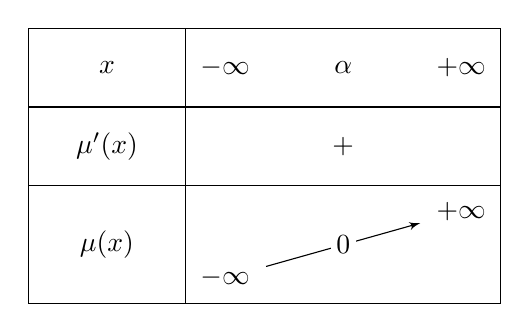
\begin{tikzpicture}
                          \tkzTabInit{$x$ /1, $\mu'(x)$ /1, $\mu(x)$ /1.5} {$-\infty$ , $+\infty$}
                          \tkzTabLine{, +,}
                          \tkzTabVar{-/$-\infty$, +/ $+\infty$}
                          \tkzTabVal{1}{2}{0.5}{$\alpha$}{0} % On place 0, son antécédent est pi / 2.
                      \end{tikzpicture}
                  \end{center}

        \end{itemize}
    \item[b)] Montrons que \( \mu(x) = 0 \) admet une unique solution dans \( ]0,1[ \)

        \textbf{Existence}

        \( \mu(0) = -1 \) et \( \mu(1) = 3 \)

        Comme \( \mu(0) \times \mu(1) < 0 \), donc \( \mu(x) = 0 \) admet une solution dans \( ]0,1[ \).

        \textbf{Unicité}

        \( \mu \) est continue et strictement croissante sur \( \mathbb{R} \), donc sur \( ]0,1[ \), \( \mu(x) = 0 \) admet une unique solution dans \( ]0,1[ \).

    \item [c)] Un encadrement de \( \alpha \) à \( 10^{-1} \) près

          \textbf{Par la méthode de balayage}

          \begin{center}
              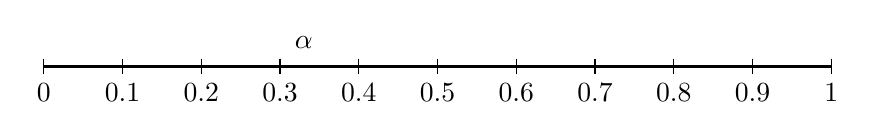
\begin{tikzpicture}
                  % Axe horizontal
                  \draw[thick] (0,0) -- (10,0);

                  % Graduations
                  \foreach \x/\val in {0/0, 1/0.1, 2/0.2, 3/0.3, 4/0.4, 5/0.5, 6/0.6, 7/0.7, 8/0.8, 9/0.9, 10/1} {
                          \draw (\x,0.1) -- (\x,-0.1) node[below] {\val};
                      }

                  % Position de alpha
                  \node[above] at (3.3,0.1) {\(\alpha\)};
              \end{tikzpicture}
          \end{center}

          \[ 0.3 \leq \alpha \leq 0.4 \]

    \item [d)] Le signe de \( \mu(x) - 1 \) pour \( \mathbb{R} \)

          \[
              \mu(x) - 1 \text{ et } \mu(x) \text{ ont les mêmes variations et mêmes limites en } -\infty \text{ et } +\infty.
          \]

          Il existe un \( \beta \) tel que  $\mu(\beta)-1 = 0$

          \begin{center}
              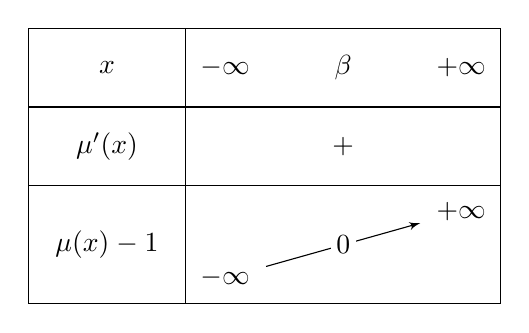
\begin{tikzpicture}
                  \tkzTabInit{$x$ /1, $\mu'(x)$ /1, $\mu(x)-1$ /1.5} {$-\infty$ , $+\infty$}
                  \tkzTabLine{, +,}
                  \tkzTabVar{-/$-\infty$, +/ $+\infty$}
                  \tkzTabVal{1}{2}{0.5}{$\beta$}{0} % On place 0, son antécédent est pi / 2.
              \end{tikzpicture}
          \end{center}
          \begin{itemize}
              \item $\forall x \in ]-\infty ; \beta[$, $\mu(x)-1 < 0 $
              \item $\forall x \in ]-\infty ; \beta[$, $\mu(x)-1 > 0 $
          \end{itemize}
\end{itemize}

\section*{Partie B}

La fonction $f$ est définie par :

\[
    f(x) =
    \begin{cases}
        \frac{2(x^3+1)}{x^2+1}, & \text{si } x < 1    \\[10pt]
        1 + \sqrt{2x -1},       & \text{si } x \geq 1
    \end{cases}
\]

\begin{enumerate}
    \item Montrer que $Df=\mathbb{R}$
          \[\text{Posons }
              f(x) =
              \begin{cases}
                  f_1(x), & \text{si } x < 1    \\[10pt]
                  f_2(x), & \text{si } x \geq 1
              \end{cases}
          \]
          \begin{itemize}
              \item[*] \( f_1 \) existe si \( x^2 + 1 \neq 0 \) et \( x < 1 \).

                  \( x \in \mathbb{R} \) et \( x < 1 \)

                  \( D_1 = ]-\infty, 1[ \)

              \item[*] \( f_2 \) existe si \( 2x -1 \geq 0 \) et \( x \geq 1 \).

                  \( 2x - 1 \geq 0 \Rightarrow x \geq \frac{1}{2} \)

                  \( x \geq \frac{1}{2} \) et \( x \geq 1 \)

                  \( x \in \left[ \frac{1}{2}, +\infty \right[ \text{ et } x\in[1, +\infty [ \)

                  \( x\in\left( \left[ \frac{1}{2}, +\infty \right[ \cap [1, +\infty [\right)  \)

                  \( x \in [1, +\infty[ \)

                  \(D_2 = [1, +\infty[\)
          \end{itemize}

          \(
          D_f = D_1 \cup D_2
          \)

          \(
          D_f = ]-\infty, 1[ \cup [1, +\infty[
          \)

          \(
          D_f = \mathbb{R}
          \)
    \item La continuité et la dérivabilité de \( f \) en 1

          \subsection*{Continuité}

          \underline{En \( 1^- \)} :

          \(
          f(x) = f_1(x) = \frac{2(x^3+1)}{x^2+1}
          \)

          \( \begin{aligned}
              \lim\limits_{x \to 1^-} f(x) & = \lim\limits_{x \to 1^-} \frac{2(x^3+1)}{x^2+1} \\
              = 2
          \end{aligned} \)

          \( \text{donc } \lim\limits_{x \to 1^-} f(x) = 2 \)

          \bigskip

          \underline{En \( 1^+ \)} :

          \( f(x) = f_2(x) = 1 + \sqrt{2x -1} \)

          \( \begin{aligned}
              \lim\limits_{x \to 1^+} f(x) & = \lim\limits_{x \to 1^+} 1 + \sqrt{2x -1} \\
                                           & = 2
          \end{aligned} \)

          \(  \text{donc } \lim\limits_{x \to 1^+} f(x) = 2 \)

          Comme
          \[
              \lim\limits_{x \to 1^-} f(x) = \lim\limits_{x \to 1^+} f(x) = f(1)
          \]
          donc \( f \) est continue en \( 1 \).

          \bigskip

          \underline{\textbf{Dérivabilité}}

          \underline{En \( 1^- \)}

          \(
          \begin{aligned}
              \lim\limits_{x \to 1^-} \frac{f(x) - f(1)}{x - 1} & = \lim\limits_{x \to 1^-} \frac{\frac{2(x^3+1)}{x^2+1} -2}{x-1}\\  
                                                                & = \lim\limits_{x \to 1^-} \frac{2x^3 +2 - 2x^2 - 2}{(x^2+1)(x-1)}\\
                                                                & = \lim\limits_{x \to 1^-} \frac{2x^3 - 2x^2}{(x^2+1)(x-1)}\\
                                                                & = \lim\limits_{x \to 1^-} \frac{2x^2 (x-1)}{(x^2+1)(x-1)}\\
                                                                & = \lim\limits_{x \to 1^-} \frac{2x^2}{(x^2+1)}\\
                                                                & = 1
          \end{aligned}
          \)
\end{enumerate}

\end{document}